% PROVENANCE (section-level)
%   status      : PRELIMINARY_RESULT
%   produced-by : Notebooks/3_fitting_cabinetry_2d_SR.ipynb (Asimov and toy
%                 pyhf/cabinetry fits, cells 36-53); the workspace files
%                 themselves are not present in this repository checkout
%                 (Appendix~\ref{app:fit:stored}), so the numbers below are
%                 the analyst's own summary of running that notebook rather
%                 than a stored, reproducible table
%   commit      : ad2f2ec
%   sample      : MC16rd + Proc16/Prompt16, Run 1 (365 fb$^{-1}$) plus
%                 partial Run 2 (125 fb$^{-1}$ processed); e and mu channels,
%                 fit separately
%   selection   : lgb_tight (Eq. lgb-tight) plus offline_cut (Eq.
%                 offline-cut); D-mass signal region plus sideband
%   corrections : PID; generic-MC luminosity 0.25; generic-BBbar weights
\section{Expected Sensitivity and Results}
\label{sec:results}

This section instead reports an Asimov (data-equals-expectation) MC sensitivity
study. The fitted data is the sum of all template samples, so the
fitted normalizations are expected to return $1$ and constrained nuisance
parameters $0$: here we determine the uncertainty on 
the $B\to D\tau\nu$ normalization (Sec.~\ref{sec:fit:poi}).

The method is described in Sec.~\ref{sec:fit:validation}: fit with every
\emph{constrained} modifier fixed while the free \texttt{normfactor}
normalizations ($D\ell\nu$, $D^{*}\ell\nu$, $D^{**}\ell\nu$~+~gap,
\texttt{bkg\_fakeD}) remain floating, to obtain the data-statistics-only
uncertainty, we then free one further constrained modifier at a time and
attribute its systematic contribution to the quadrature difference between
the new and previous returned uncertainty.
Electron and muon channels are fit separately, each against its own
two-channel (signal region plus sideband) workspace. The two resulting
uncertainties are combined at the end (below) rather than fit jointly.

\begin{table}[htbp]
  \centering
  \caption{Preliminary Asimov-sensitivity breakdown on the $B\to D\tau\nu$
  normalization, by channel. ``Data statistics only'' fixes every
  constrained (\texttt{normsys}/\texttt{staterror}) modifier while the free
  \texttt{normfactor} normalizations ($D\ell\nu$, $D^{*}\ell\nu$,
  $D^{**}\ell\nu$~+~gap, \texttt{bkg\_fakeD}) remain floating
  (Sec.~\ref{sec:fit:validation}); each subsequent row is the quadrature
  difference introduced by freeing one further constrained modifier relative
  to the row above, with one exception: the $D^{*}\tau\nu$ and $D^{**}\tau\nu$
  \texttt{normsys} modifiers are freed together as a single joint step rather
  than one at a time, so that row's $\pm4.6\%$ is their combined
  contribution, not either modifier's individually; ``more systematics''
  denotes contributions not yet enabled in the fit (Sec.~\ref{sec:syst}).
  The ``Total'' row is the uncertainty returned directly by the fit with all
  listed modifiers simultaneously free, not a value recomputed from the rows
  above: summing the four individual differences in quadrature gives
  $14.1\%$ ($e$) and $21.8\%$ ($\mu$).}
  \vspace{2mm}
  \label{tab:sensitivity-breakdown}
  \small
  \begin{tabular}{l c c}
    \hline
    Contribution & $e$ channel & $\mu$ channel \\
    \hline
    Data statistics only & $11.8\%$ & $19.1\%$ \\
    $+$ norm.\ sys.\ ($D^{*}\tau\nu$ \& $D^{**}\tau\nu$, joint) & $\pm 4.6\%$ & $\pm 4.6\%$ \\
    $+$ norm.\ sys.\ (continuum) & $\pm 2.4\%$ & $\pm 1.3\%$ \\
    $+$ MC statistics (\texttt{staterror}) & $\pm 5.8\%$ & $\pm 9.3\%$ \\
    $+$ more systematics (not yet enabled) & \multicolumn{2}{c}{---} \\
    \hline
    \textbf{Total, this channel} & $\gtrsim 14.5\%$ & $\gtrsim 22.1\%$ \\
    \hline
  \end{tabular}
\end{table}


\paragraph{Combination.}
The electron channel is more sensitive than the muon
channel: the tighter muon momentum requirement and the KLM acceptance ($p_{\mu} > 0.6$\,GeV$/c$
versus $p_{e} > 0.3$\,GeV$/c$, Sec.~\ref{sec:reconstruction}) removes a larger
fraction of $B\to D\tau\nu$ signal. The signal lepton momentum
spectrum peaks at low momentum, giving the muon channel roughly half the
signal-enriched $D\tau\nu$ statistics of the electron channel
(Table~\ref{tab:sensitivity-sample-sizes}).
The two channels' uncertainties are combined as an inverse-variance-weighted
average, $\sigma_{\rm comb} = \left(\sigma_{e}^{-2} +
\sigma_{\mu}^{-2}\right)^{-1/2}$, which gives $\sigma_{\rm comb} = 12.1\%$
for $14.5\%$ and $22.1\%$ above, which gives
$12.2\%$ (a $0.1$ percentage-point difference).

Systematic correlations between the electron and muon channels have been neglected so far.





% PROVENANCE
%   status      : PRELIMINARY_RESULT
%   produced-by : same Asimov fit as the table above (electron channel)
%   commit      : ad2f2ec
%   sample      : as above, e channel
%   selection   : as above
%   corrections : as above
\begin{figure}[htbp]
  \centering
  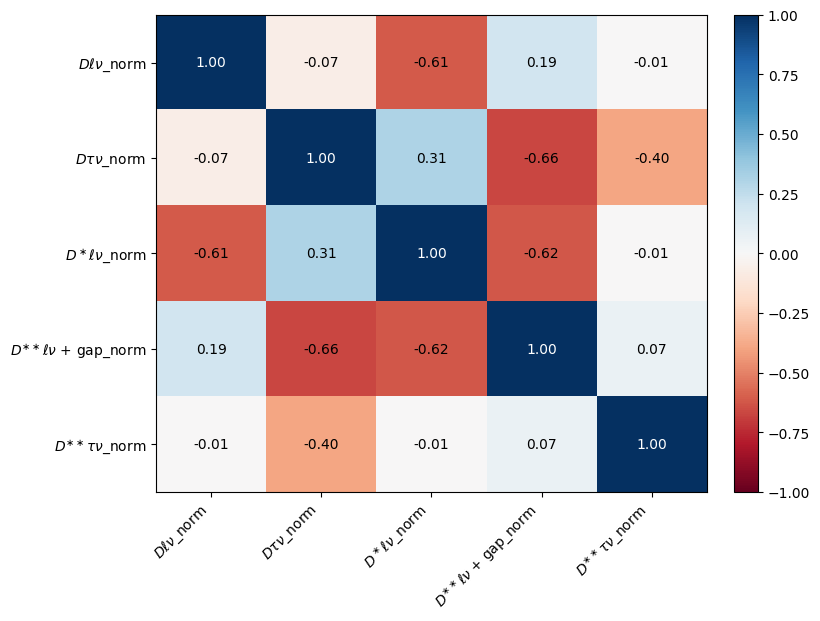
\includegraphics[width=0.7\textwidth]{pyhf_fit_correlation.png}
  \caption{Correlation matrix of five fitted normalization parameters from
  the electron-channel Asimov fit, produced by
  \texttt{cabinetry.visualize.correlation\_matrix(fit\_results,
  pruning\_threshold=0.3)}.
  Four are free \texttt{normfactor} parameters ($D\ell\nu$, $D\tau\nu$,
  $D^{*}\ell\nu$, $D^{**}\ell\nu$~+~gap); the fifth, $D^{**}\tau\nu$\_norm, is
  a constrained \texttt{normsys} parameter (Table~\ref{tab:fit-parameters})
  included because it correlates with at least one other shown parameter
  above the threshold (0.3).
  The parameter of interest, $D\tau\nu$\_norm, is most anti-correlated with
  $D^{**}\ell\nu$~+~gap\_norm ($\rho=-0.66$) and $D^{**}\tau\nu$\_norm
  ($\rho=-0.40$), and positively correlated with $D^{*}\ell\nu$\_norm
  ($\rho=0.31$): the
  categories whose $\mmiss$/$\pdl$ shapes most resemble $D\tau\nu$ are also
  the ones most correlated with its fitted normalization.}
  \label{fig:pyhf-correlation}
\end{figure}

